\documentclass[letterpaper,12pt]{article}

\usepackage{threeparttable}
\usepackage{geometry}
\geometry{letterpaper,tmargin=1in,bmargin=1in,lmargin=1.25in,rmargin=1.25in}
\usepackage[format=hang,font=normalsize,labelfont=bf]{caption}
\usepackage{amsmath}
\usepackage{mathrsfs}
\usepackage{multirow}
\usepackage{array}
\usepackage{delarray}
\usepackage{listings}
\usepackage{amssymb}
\usepackage{amsthm}
\usepackage{lscape}
\usepackage{natbib}
\usepackage{setspace}
\usepackage{float,color}
\usepackage[pdftex]{graphicx}
\usepackage{pdfsync}
\usepackage{verbatim}
\usepackage{placeins}
\usepackage{geometry}
\usepackage{pdflscape}
\synctex=1
\usepackage{hyperref}
\hypersetup{colorlinks,linkcolor=red,urlcolor=blue,citecolor=red}
\usepackage{bm}


\theoremstyle{definition}
\newtheorem{theorem}{Theorem}
\newtheorem{acknowledgement}[theorem]{Acknowledgement}
\newtheorem{algorithm}[theorem]{Algorithm}
\newtheorem{axiom}[theorem]{Axiom}
\newtheorem{case}[theorem]{Case}
\newtheorem{claim}[theorem]{Claim}
\newtheorem{conclusion}[theorem]{Conclusion}
\newtheorem{condition}[theorem]{Condition}
\newtheorem{conjecture}[theorem]{Conjecture}
\newtheorem{corollary}[theorem]{Corollary}
\newtheorem{criterion}[theorem]{Criterion}
\newtheorem{definition}{Definition} % Number definitions on their own
\newtheorem{derivation}{Derivation} % Number derivations on their own
\newtheorem{example}[theorem]{Example}
\newtheorem{exercise}[theorem]{Exercise}
\newtheorem{lemma}[theorem]{Lemma}
\newtheorem{notation}[theorem]{Notation}
\newtheorem{problem}[theorem]{Problem}
\newtheorem{proposition}{Proposition} % Number propositions on their own
\newtheorem{remark}[theorem]{Remark}
\newtheorem{solution}[theorem]{Solution}
\newtheorem{summary}[theorem]{Summary}
\bibliographystyle{aer}
\newcommand\ve{\varepsilon}
\renewcommand\theenumi{\roman{enumi}}
\newcommand\norm[1]{\left\lVert#1\right\rVert}

\begin{document}

\title{Econ 581 Homework 6}
\author{Chris Rytting}
\maketitle
\subsection*{Exercise 1}


\subsection*{Paths}


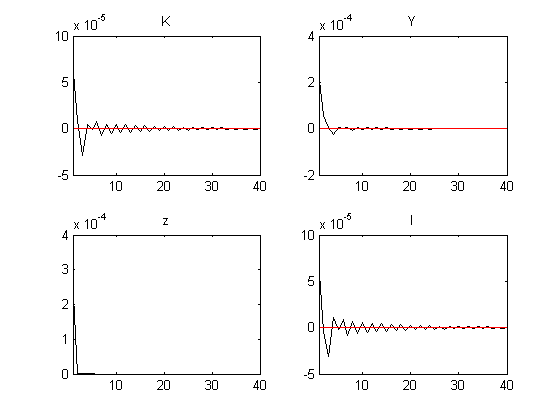
\includegraphics[scale = .8]{ans1}\\

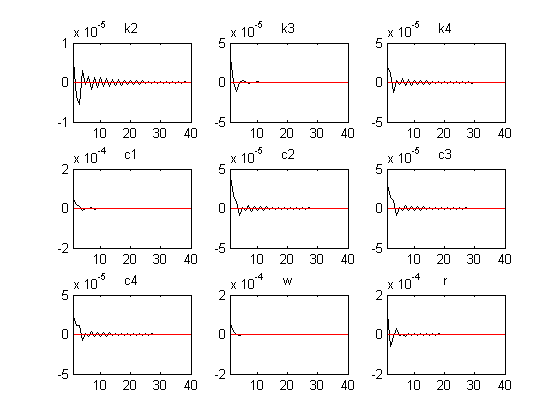
\includegraphics[scale = .8]{ans2}\\

\subsection*{SS Results}



k2 	=	 0.117727\\
k3 	=	 0.278812\\
k4 	=	 0.178062\\
c1 	=	 0.285387\\
c2 	=	 0.247752\\
c3 	=	 0.215081\\
c4 	=	 0.186718\\
w  	=	 0.403114\\
r  	=	 0.84996\\
K  	=	 0.574602\\
Y  	=	 1.39539\\
z  	=	 0\\
I  	=	 0.460458\\



\subsection*{Model Summary}



  Number of variables:         13\\
  Number of stochastic shocks: 1\\
  Number of state variables:   5\\
  Number of jumpers:           1\\
  Number of static variables:  7\\


\[
\begin{matrix}
Simulated variables moments:\\
Variable &Mean &   Std. Dev.  & Variance &  Skewness &  Kurtosis\\ 
k2& 0.117727 &  0.000012&   0.000000 &  0.007672 & -0.343016\\
k3     &      0.278810  & 0.000039   &0.000000   &0.130038  & 0.379393\\
k4    &       0.178061   &0.000033   &0.000000  &-0.108399  & 0.525654\\
c1   &        0.285381   &0.000069   &0.000000   &0.182404  &-0.173503\\
c2          & 0.247747   &0.000056   &0.000000   &0.193003  &-0.144669\\
c3         &  0.215077   &0.000046   &0.000000   &0.198076  &-0.056893\\
c4        &   0.186714   &0.000038   &0.000000   &0.195721  & 0.093621\\
w        &    0.403108  & 0.000071   &0.000000   &0.158804  &-0.117236\\
r       &     0.849954  & 0.000144   &0.000000   &0.214612   &0.232132\\
K      &      0.574598  & 0.000076   &0.000000  &-0.077032   &0.193026\\
Y     &       1.395374  & 0.000247   &0.000000   &0.158804  &-0.117236\\
z        &   -0.000018   &0.000250   &0.000000   &0.160410   &0.097716\\
I       &     0.460455   &0.000077   &0.000000  &-0.063740  &-0.021642\\
\end{matrix}
\]

\[\begin{matrix}
Autocorrelation\\
Variable  &    1  &     2    &   3     &  4  &     5   \\
k2  &       -0.3577 &-0.0369 &-0.3528 & 0.3249 &-0.1989\\
k3   &       0.1019 &-0.3399 &-0.2431 & 0.0505 & 0.0760\\
k4    &     -0.1877 & 0.1035 &-0.5023 & 0.3156 &-0.2306\\
c1     &     0.1447 & 0.1063 &-0.4419 & 0.1145 &-0.1244\\
c2      &    0.0834 & 0.1933 &-0.4904 & 0.1687 &-0.1871\\
c3       &   0.0026 & 0.2903 &-0.5459 & 0.2360 &-0.2608\\
c4 &        -0.0969 & 0.3905 &-0.6054 & 0.3147 &-0.3418\\
w   &        0.1826 &-0.0020 &-0.3614 & 0.0558 &-0.0560\\
r    &      -0.2841 &-0.1188 &-0.0234 & 0.1124 &-0.1111\\
K     &      0.0403 &-0.2700 &-0.2800 & 0.0948 & 0.0278\\
Y      &     0.1826 &-0.0020 &-0.3614 & 0.0558 &-0.0560\\
z       &    0.0302 &-0.0052& -0.2463 & 0.0712 &-0.0890\\
I        &  -0.0987 &-0.2278& -0.2505 & 0.1467 &-0.0284\\
\end{matrix}\]










\end{document}
